\chapter{Драйвер SPI устройства}
\textbf{Цель:} Активировать SPI контроллер, и написать простой драйвер для устройства подключённого к SPI интерфейсу.

\vspace{5mm}
\textbf{Описание:}В данной работе, познакомимся со структурой ядра, позволяющей взаимодействовать с spi контроллером целевой платы. Данная структура является программным интерфейсом, позволяющим отвязать реализацию взаимодействия с внешним аппаратным модулем по интерфейсу SPI от особенностей реализации SPI контроллера на конкретной аппаратной платформе. 

\vspace{5mm}
\textbf{Полезные ссылки:}
\begin{itemize}
	\item \href{http://www.gaw.ru/html.cgi/txt/interface/spi/index.htm}{Последовательный интерфейс SPI}.
	\item \href{https://docs.kernel.org/devicetree/dynamic-resolution-notes.html}{Kernel Doc: Devicetree Dynamic Resolver Notes}
	\item \href{https://www.kernel.org/doc/html/v4.15/driver-api/spi.html}{Kernel Doc: SPI API}	
\end{itemize}

\section{Запуск и подключение к устройству}

\subsection{}Запустите виртуальную машину. Логин и пароль для входа: student / usrstudent.

\subsection{}Подключите по USB плату к ПК. Проверьте, и при необходимости подключите USB устройство FTDI RBM\_C1K5500VK018 к виртуальной машине (меню Device→USB).

\subsection{}Откройте программу gtkterm, и подключитесь к порту /dev/ttyUSB1

\subsection{}Если в окне терминала нет текста, нажмите клавишу Enter на клавиатуре. Вы должны увидеть следующий вывод:
\begin{center}
	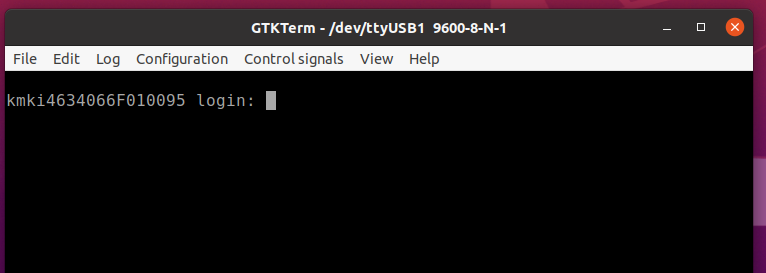
\includegraphics[width=\textwidth]{pic_08}
\end{center}
Вы подключились к консоли устройства. Введите логин root и пароль root.


\section{Подготовка Device Tree Overlay}
Основная конфигурация целевой платы предполагает, что практически все выводы настроены для управления через блок GPIO. Для работы с SPI, нам необходимо ввести две правки: разрешить работу SPI контроллера и передать под его управления выводы, для коммуникации с внешним миром. 

\subsection{} Создадим рабочую папку в виртуальной машине для создания device-tree overlay и перейдём в неё 
\begin{lstlisting}[style=bash]
# mkdir -p $BAGET/lab_05/devtree
# cd $BAGET/lab_05/devtree
\end{lstlisting}

\subsection{}Создадим новый файл
\begin{lstlisting}[style=bash]
# kate of_spi1.dts
\end{lstlisting}
и запишем в него следующий текст
\begin{lstlisting}[style=stdout]
/dts-v1/;
/plugin/;
/ {
	fragment@0 {
		target-path = "/gpio@1b400200";
		
		__overlay__ {
			
			spi1_pins {
				phandle = <0x01>;
				
				spi1_clk {
					function = "spi1_clk";
					groups = "spi1_clk";
				};
				
				spi1_di {
					function = "spi1_di";
					groups = "spi1_di";
				};
				
				spi1_do {
					function = "spi1_do";
					groups = "spi1_do";
				};
				
				spi1_cs0 {
					function = "spi1_cs0";
					groups = "spi1_cs0";
				};
			};
		};
	};
	
	
	fragment@1 { 
		target-path = "/spi@1a800000"; 
		
		__overlay__ { 
			status = "okay"; 
			pinctrl-names = "default"; 
			pinctrl-0 = <0x01>; 
		}; 
	}; 
	
	
	__local_fixups__ {
		
		fragment@1 {
			__overlay__ {
				pinctrl-0 = <0x00>;
			};
		};
		
	};
};
\end{lstlisting}

Разберём, что мы тут создали. Данное дополнение состоит из нескольких фрагментов, так как переписать нам нужно две разные ноды, однако изменения эти должны быть синхронизированы между собой, по этой причине они находятся в одном файле. 

Первый фрагмент, это дополнение к ноде описывающей банк выводов А. В этом дополнении мы создаём конфигурацию, для передачи управления частью выводов SPI контроллеру. Будьте внимательны, не любой вывод может быть передан SPI контроллеру. 

Следующий фрагмент правок, касается дополнения к описанию spi контроллера. Первое, это его активация, записью в параметр status значения okay. Так же, мы вводим два дополнительных параметра, один хранит в себе название конфигурации выводов, второй — для указания идентификатора конфигурации, обратите внимание, что значение у него совпадает (и это важно) со значением phandle у описания выводов из первого фрагмента.

Последняя строка гарантирует, что после применения этого дополнения, значение параметра pinctrl-0 будет соответствовать значению phandle нашей группы spi1\_pins. Дело в том, что значение phandle из первого фрагмента, будет  актуализировано, для разрешения коллизий (так как в исходном device-tree уже есть нода, с таким значением phandle), и последняя строка в нашем описании исправлений поясняет системе, что после разрешения коллизии, необходимо обновить значение указанного параметра (значение 0 зарезервировано, и в данном контексте означает ссылку на значение параметра phandle).  

Узнать, какой банк выводов, и какие выводы могут быть использованы с тем или иным интерфейсом, какие значения phandle уже использованы, и просто для любопытства можно одним из двух способов:

\begin{enumerate}
	\item Из самой системы, изучив подкаталоги gpio, в каталоге /proc/device-tree/ (рекомендуется для считывания значение того или иного параметра использовать команду cat). 
	
	\item Преобразовав бинарный файл device-tree системы в текстовый вид 
	\begin{lstlisting}[style=bash]
	# dtc --symbol -O -dts -o  /tmp/root.dts \
	$BAGET/support/barebox/k5500vk018_rbm.dts
	# kate /tmp/root.dts
	\end{lstlisting}
\end{enumerate}

Посмотрите на ноды, описывающие банки GPIO выводов. Так же обратите внимание, на объявление конфигураций выводов для sdhci контроллера, особенно, как эта конфигурация разбита, между двумя банками выводов, на значение параметра phandle каждой группы. Сравните значение параметров phandle конфигурационных груп, и значения перечисленные в параметре pinctrl-0 у ноды для контроллера  sdhci. (не стесняйтесь использовать поиск по файлу).

\subsection{}Сохраните изменения Ctrl+S и закройте редактор Ctrl+Q 

\subsection{}Скомпилируем файл и скопируем его на плату
\begin{lstlisting}[style=bash]
# dtc --symbol -O dtb -o ./of_spi1.dtb ./of_spi1.dts
# scp ./of_spi1.dtb netuser@192.168.100.200:/home/netuser/
\end{lstlisting}

\subsection{}Перейдите в терминал платы, и переместите файл в папку barebox
\begin{lstlisting}[style=bash]
$ mv /home/netuser/of_spi1.dtb /barebox/
\end{lstlisting}

\subsection{}Откройте скритп barebox.sh для редактирования
\begin{lstlisting}[style=bash]
$ nano /barebox/barebox.sh
\end{lstlisting}

\subsection{}Впишите после строки DTB=k5500vk018\_rbm.dtb следующую строчку (при наличии других строк, закомментируйте их символом \# )
\begin{lstlisting}[style=stdout]
fdt_apply -i $DTB -l of_spi1.dtb -o /dtb && DTB=/dtb
\end{lstlisting}
Сохраним изменения и выйдем из редактора (Ctrl+S, Ctrl+X)

\subsection{}Перезагрузите плату командой reboot. 

\subsection{}После перезагрузки входим в систему (root/root). И выполняем команду
\begin{lstlisting}[style=bash]
$ ls /sys/class/spi_master/
\end{lstlisting}
Вы должны увидеть, два имени: spi0 (это контроллер qspi flash-памяти) и spi1 (тот что мы активировали). Если второго имени нет, значит дополнение к device-tree не отработало. Проверьте, что Вы правильно написали команду в файле /barebox/barebox.sh, а так же изучите вывод платы во время загрузки. 

\section{Собираем драйвер}
В Linux есть драйвер для управления spi контроллером из пространства пользоватея, он называется spidev. Однако у него есть ряд недостатков, которые мешают использовать его в боевых проектах. В системе целевой платы этот драйвер отсутствует, и посмотреть на его работу мы не сможем. Поэтому сразу же начнём собирать свой драйвер.

\subsection{}Подготовим папку для сборки драйвера, перейдём в неё и откроем в редакторе vscode
\begin{lstlisting}[style=bash]
# cp -r $BAGET/support/spi_driver $BAGET/lab_05/driver 
# cd $BAGET/lab_05/driver; code .
\end{lstlisting}
\textbf{Замечание:} При первом входе, Вас могут спросить, доверяете ли вы автору, нужно нажать на кнопку Yes,  
\begin{center}
	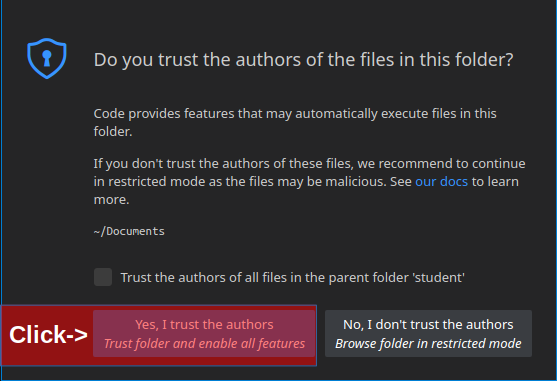
\includegraphics[width=0.5\textwidth]{pic_13}
\end{center}

\subsection{}Добавим путей для разрешения части include директив. Откройте .vscode -> c\_cpp\_properties.json
\begin{center}
	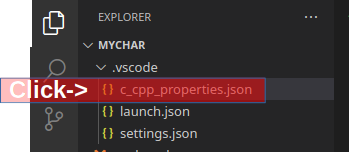
\includegraphics[width=0.5\textwidth]{pic_14}
\end{center}

\subsection{}Допишите в поле includePath следующие строки:\\
\begin{center}
	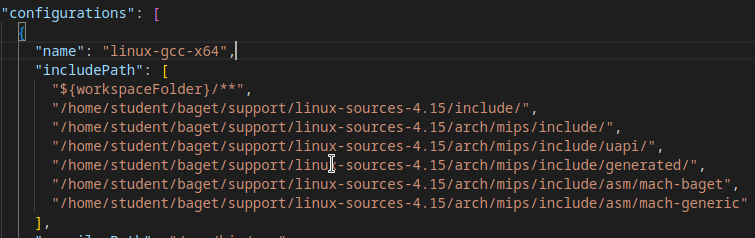
\includegraphics[width=\textwidth]{pic_15}
\end{center}
для удобства, воспользуйтесь файлом vscode\_lines.md в папке support. Ctrl+S для сохранения.

\subsection{}Изучите исходны код в файле spi\_temp.c. Для работы с SPI интерфейсом, в Linux есть готовые структуры, которые в данной работе используются. 

Из особенностей, которые хотелось бы отметить, это структура описание которой начинается с 11 строки. В ней описывается режим работы SPI интерфейса, в том числе номер интерфейса в системе. В нашем случае 1, так как 0 будет занят контроллером QSPI памяти.

Так же обратите внимание на организацию транзакции, описанную в функции  ext\_spi\_write (начало описания с 28 строки). В ней используется структура spi\_transfer, информацию о которой Вы можете получить, перейдя по ссылке 3 приведённой в начале лабораторной работы.

\subsection{}Перейдём в терминал (можно открыть вкладку TERMINAL в vscode, если её не видно, выберите в меню Terminal → New Terminal) и соберём модуль командой
\begin{lstlisting}[style=bash]
# ARCH=mips CROSS_COMPILE=mips64el-linux-gnuabi64- make 
\end{lstlisting}

\subsection{}Перейдём в терминал (можно открыть вкладку TERMINAL в vscode, если её не видно, выберите в меню Terminal → New Terminal) и соберём модуль командой
\begin{lstlisting}[style=bash]
	# ARCH=mips CROSS_COMPILE=mips64el-linux-gnuabi64- make 
\end{lstlisting}

\subsection{}Проверьте значение системной переменной BRD\_PASS  
\begin{lstlisting}[style=bash]
	# echo $BRD_PASS
\end{lstlisting}
если вывод был пустой, проинициализируйте переменную 
\begin{lstlisting}[style=bash]
	# export BRD_PASS="usrnetuser" 
\end{lstlisting}

\subsection{}Скопируйте модуль на плату
\begin{lstlisting}[style=bash]
	# ARCH=mips CROSS_COMPILE=mips64el-linux-gnuabi64- make install
\end{lstlisting}

\subsection{}Подключите модуль PmodALS как показано на рисунке 
\begin{center}
	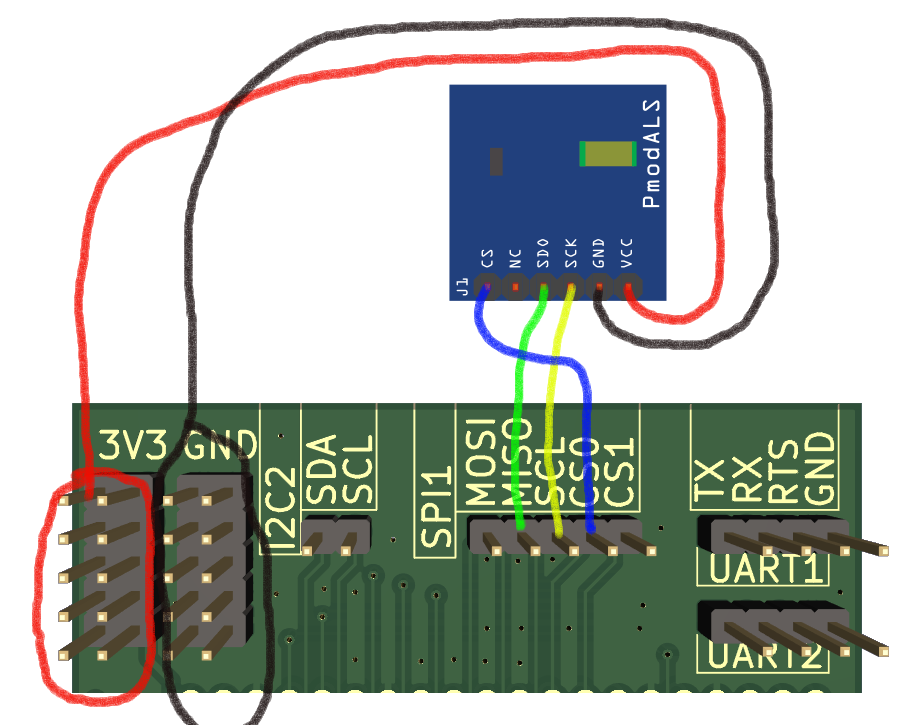
\includegraphics[width=0.7\textwidth]{pic_20}
\end{center}

\subsection{}Перейдите в терминал платы, и активируйте драйвера
\begin{lstlisting}[style=bash]
$ insmod /home/netuser/spi_temp.ko 
\end{lstlisting}

\subsection{}Вы должны увидите в терминале, информацию о том, что драйвер зарегистрирован, и 10 раз считано «сырое» значение освещённости с датчика.

\subsection{}Выгрузите драйвер командой
\begin{lstlisting}[style=bash]
$ rmmod spi_temp
\end{lstlisting}

\subsection{} Выключите плату, для чего в начале введите команду
\begin{lstlisting}[style=bash]
	$ poweroff
\end{lstlisting}
дождитесь, как появиться надпись
\begin{lstlisting}[style=stdout]
	reboot: System halt
\end{lstlisting}
после чего отключите USB кабель от ПК или платы. 

\section{Задание для самостоятельной работы}
Внесите изменения в текущий драйвер таким образом, что бы создавался файл в папке /dev, чтение которого давало бы текущее значение освещённости.

В этом Вам может помочь код из лабораторной работы \ref{lab:char_dev}.

\subsubsection{*}
Внесите изменение в драйвер устройств таким образом, что бы частота, номер spi шины, и индекс вывода Chip Select передавались через описание в дереве устройств:
\begin{lstlisting}[style=stdout]
pmodals {
	compatible = "digilent,pmodals";
	spi_cfg = <400000 1 0>;	  
	status = "okay";
};
\end{lstlisting}